% !TEX TS-program = pdflatex
\documentclass[11pt]{article}

% -------------------- Packages --------------------
\usepackage[a4paper,margin=1in]{geometry}
\usepackage{amsmath,amssymb}
\usepackage[T1]{fontenc}
\usepackage{lmodern}
\usepackage{xcolor}
\usepackage{tcolorbox}
\tcbuselibrary{skins,breakable}
\usepackage{enumitem}
\usepackage{hyperref}
\usepackage{tikz}
\usetikzlibrary{calc,angles,quotes,arrows.meta}

\pagestyle{empty}

% -------------------- Dark Theme Colors --------------------
\definecolor{bg}{HTML}{000000}
\definecolor{pairbg}{HTML}{121212}
\definecolor{solbg}{HTML}{0A0A0A}
\definecolor{border}{HTML}{2A2A2A}
\definecolor{text}{HTML}{FFFFFF}
\definecolor{muted}{HTML}{C9CDD3}
\definecolor{gold}{HTML}{FFD700}
\definecolor{green}{HTML}{4ADE80}
\definecolor{cyan}{HTML}{38BDF8}

\pagecolor{bg}
\color{text}

\hypersetup{
  colorlinks=true,
  linkcolor=cyan,
  urlcolor=cyan
}

\setlength{\parindent}{0pt}
\setlength{\parskip}{10pt}

% Help LaTeX avoid overfull lines globally
\sloppy
\setlength{\emergencystretch}{3em}

\setlist[itemize]{left=1.4em,itemsep=6pt,topsep=6pt}
\setlist[enumerate]{left=1.6em,itemsep=4pt,topsep=4pt}

% -------------------- tcolorbox Base --------------------
\tcbset{
  enhanced,
  breakable,
  arc=12pt,
  boxrule=0.8pt,
  left=14pt,right=14pt,top=12pt,bottom=12pt
}

\newtcolorbox{QAPair}[1]{%
  colback=pairbg,
  colbacklower=solbg,
  colframe=border,
  coltext=text,
  title=\textcolor{gold}{\bfseries #1},
  fonttitle=\bfseries,
  coltitle=text,
  segmentation style={draw=border, dashed, line width=0.6pt},
  before upper=\raggedright,
  before lower=\raggedright
}

\newtcolorbox{QuickBox}{%
  colback=pairbg,
  colframe=cyan,
  coltext=text,
  fontupper=\color{text}\raggedright,
  borderline north={4pt}{0pt}{cyan},
  arc=14pt,
  boxrule=0.8pt
}

% Helper for step headings
\newcommand{\Step}[1]{\textcolor{muted}{\textbf{Step #1:}}}

% Small centered diagram block
\newenvironment{StepDiagram}{\par\medskip\begin{center}}{\end{center}\medskip}

% TikZ styles
\tikzset{
  base/.style={draw=text, line width=0.9pt, line cap=round, line join=round},
  new/.style={draw=cyan, line width=1.2pt, line cap=round, line join=round},
  help/.style={draw=muted, dashed, line width=0.9pt},
  ang/.style={draw=gold, line width=1.0pt},
  dot/.style={circle, fill=text, inner sep=1.2pt},
  lab/.style={text=text, font=\small},
  labm/.style={text=muted, font=\small},
  labfill/.style={lab, fill=pairbg, inner sep=1.2pt}
}

% A tiny "equation diagram" (boxed working) to prevent overflow
\newcommand{\EqDiagram}[1]{%
\begin{StepDiagram}
\begin{tikzpicture}
\node[draw=border, rounded corners=10pt, inner sep=8pt, text=text, align=left, text width=0.88\linewidth] {#1};
\end{tikzpicture}
\end{StepDiagram}
}

% ============================================================
\begin{document}

\begin{center}
{\LARGE\bfseries \textcolor{gold}{Miscellaneous Exercise 9 --- Solutions}}\\[-2pt]
\end{center}

% -------------------- Quick facts (each line has its own diagram) --------------------
\begin{QuickBox}
{\color{cyan}\bfseries Quick facts}\par\medskip

\textcolor{gold}{\bfseries (1) Unique circle:} Exactly one circle passes through \textbf{3 non-collinear points}.
\begin{StepDiagram}
\begin{tikzpicture}[scale=0.95]
  \def\R{1.55}
  \coordinate (O) at (0,0);
  \coordinate (A) at ({\R*cos(40)},{\R*sin(40)});
  \coordinate (B) at ({\R*cos(160)},{\R*sin(160)});
  \coordinate (C) at ({\R*cos(260)},{\R*sin(260)});
  \draw[base] (O) circle (\R);
  \node[dot] at (A) {};
  \node[dot] at (B) {};
  \node[dot] at (C) {};
  \node[lab] at ($(A)+(0.20,0.12)$) {$A$};
  \node[lab] at ($(B)+(-0.20,0.12)$) {$B$};
  \node[lab] at ($(C)+(0,-0.22)$) {$C$};
  \node[labm] at (0,-2.05) {3 non-collinear points determine one circle};
\end{tikzpicture}
\end{StepDiagram}

\textcolor{gold}{\bfseries (2) Perpendicular from centre:} If a line through the centre is \textbf{perpendicular} to a chord, it \textbf{bisects} the chord.
\begin{StepDiagram}
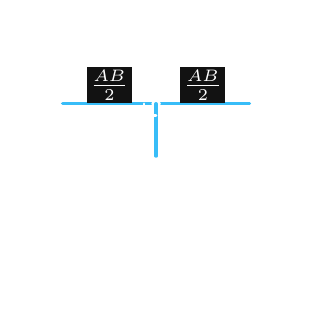
\begin{tikzpicture}[scale=0.95]
  \def\r{1.7}
  \coordinate (O) at (0,0);
  \coordinate (A) at (-1.25,0.70);
  \coordinate (B) at ( 1.25,0.70);
  \coordinate (M) at ($(A)!0.5!(B)$);
  \draw[base] (O) circle (\r);
  \node[dot,label={[lab]below:$O$}] at (O) {};
  \draw[new] (A)--(B);
  \node[dot] at (M) {};
  \node[lab] at ($(M)+(0,0.25)$) {$M$};
  \draw[new] (O)--(M);
  \draw[base] ($(M)+(-0.16,0)$) -- ($(M)+(-0.16,-0.16)$) -- ($(M)+(0,-0.16)$);
  \node[labfill] at ($(A)!0.5!(M)+(0,0.25)$) {$\frac{AB}{2}$};
  \node[labfill] at ($(M)!0.5!(B)+(0,0.25)$) {$\frac{AB}{2}$};
\end{tikzpicture}
\end{StepDiagram}

\textcolor{gold}{\bfseries (3) Chord distance formula:} If radius $r$ and chord length $L$, distance from centre is
\[
d=\sqrt{r^2-\left(\frac{L}{2}\right)^2}.
\]
\begin{StepDiagram}
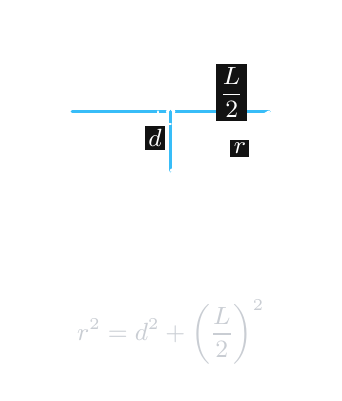
\begin{tikzpicture}[scale=1.00]
  \def\r{1.8}
  \coordinate (O) at (0,0);
  \coordinate (A) at (-1.25,0.75);
  \coordinate (B) at ( 1.25,0.75);
  \coordinate (M) at ($(A)!0.5!(B)$);

  \draw[base] (O) circle (\r);
  \node[dot] at (O) {};
  \node[lab] at ($(O)+(0,-0.25)$) {$O$};

  \draw[new] (A)--(B);
  \node[dot] at (M) {};
  \node[lab] at ($(M)+(0,0.26)$) {$M$};

  \draw[new] (O)--(M);
  \draw[base] (O)--(B);

  \draw[base] ($(M)+(-0.16,0)$) -- ($(M)+(-0.16,-0.16)$) -- ($(M)+(0,-0.16)$);

  \node[labfill] at ($(O)!0.55!(M)+(-0.20,0)$) {$d$};
  \node[labfill] at ($(M)!0.62!(B)+(0,0.24)$) {$\dfrac{L}{2}$};
  \node[labfill] at ($(O)!0.56!(B)+(0.18,-0.14)$) {$r$};

  \node[labm] at (0,-2.05) {$r^2=d^2+\left(\dfrac{L}{2}\right)^2$};
\end{tikzpicture}
\end{StepDiagram}

\textcolor{gold}{\bfseries (4) Chord length at distance $d$:}
\[
L=2\sqrt{r^2-d^2}.
\]
\begin{StepDiagram}
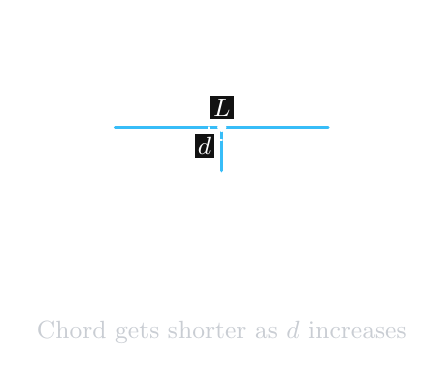
\begin{tikzpicture}[scale=1.00]
  \def\r{1.8}
  \coordinate (O) at (0,0);
  \coordinate (A) at (-1.35,0.55);
  \coordinate (B) at ( 1.35,0.55);
  \coordinate (M) at ($(A)!0.5!(B)$);

  \draw[base] (O) circle (\r);
  \node[dot,label={[lab]below:$O$}] at (O) {};
  \draw[new] (A)--(B);
  \draw[new] (O)--(M);
  \node[dot] at (M) {};
  \node[lab] at ($(M)+(0,0.25)$) {$M$};

  \draw[base] ($(M)+(-0.16,0)$) -- ($(M)+(-0.16,-0.16)$) -- ($(M)+(0,-0.16)$);

  \node[labfill] at ($(O)!0.58!(M)+(-0.22,0)$) {$d$};
  \node[labfill] at ($(A)!0.5!(B)+(0,0.25)$) {$L$};
  \node[labm] at (0,-2.05) {Chord gets shorter as $d$ increases};
\end{tikzpicture}
\end{StepDiagram}

\textcolor{gold}{\bfseries (5) Central angles:} Full circle $=360^\circ$, semicircle $=180^\circ$, quadrant $=90^\circ$.

\begin{StepDiagram}
\begin{tikzpicture}[scale=0.92]
  \def\R{1.55}
  \coordinate (O) at (0,0);
  \coordinate (A) at (\R,0);
  \coordinate (B) at (0,\R);
  \coordinate (C) at (-\R,0);
  \draw[base] (O) circle (\R);
  \node[dot,label={[lab]below:$O$}] at (O) {};
  \draw[new] (O)--(A);
  \draw[new] (O)--(B);
  \pic[ang,"$90^\circ$",lab,angle radius=8mm,angle eccentricity=1.15] {angle=A--O--B};
  \node[labm] at (0,-2.00) {Quadrant};
\end{tikzpicture}
\end{StepDiagram}

\begin{StepDiagram}
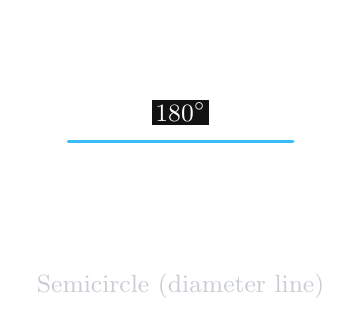
\begin{tikzpicture}[scale=0.92]
  \def\R{1.55}
  \coordinate (O) at (0,0);
  \coordinate (A) at (\R,0);
  \coordinate (C) at (-\R,0);
  \draw[base] (O) circle (\R);
  \node[dot,label={[lab]below:$O$}] at (O) {};
  \draw[new] (O)--(A);
  \draw[new] (O)--(C);
  \node[labfill] at (0,0.40) {$180^\circ$};
  \node[labm] at (0,-2.00) {Semicircle (diameter line)};
\end{tikzpicture}
\end{StepDiagram}

\begin{StepDiagram}
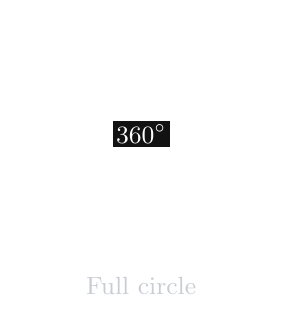
\begin{tikzpicture}[scale=0.92]
  \def\R{1.55}
  \coordinate (O) at (0,0);
  \draw[base] (O) circle (\R);
  \node[dot,label={[lab]below:$O$}] at (O) {};
  \node[labfill] at (0,0.10) {$360^\circ$};
  \node[labm] at (0,-2.00) {Full circle};
\end{tikzpicture}
\end{StepDiagram}

\end{QuickBox}

% ============================================================
\begin{QAPair}{MCQ (i)}
\textcolor{gold}{\bfseries Question:} One and only one circle can pass through \_\_\_\_\_ non-collinear points.\\
(a) 2 \quad (b) 3 \quad (c) 4 \quad (d) 5
\tcblower
\textcolor{green}{\bfseries Answer:}\par
\Step{1} A unique circle is determined by \textbf{three} non-collinear points.
\begin{StepDiagram}
\begin{tikzpicture}[scale=0.90]
  \def\R{1.55}
  \coordinate (O) at (0,0);
  \coordinate (A) at ({\R*cos(30)},{\R*sin(30)});
  \coordinate (B) at ({\R*cos(150)},{\R*sin(150)});
  \coordinate (C) at ({\R*cos(250)},{\R*sin(250)});
  \draw[base] (O) circle (\R);
  \node[dot] at (A) {};
  \node[dot] at (B) {};
  \node[dot] at (C) {};
  \node[lab] at ($(A)+(0.22,0.10)$) {$A$};
  \node[lab] at ($(B)+(-0.22,0.10)$) {$B$};
  \node[lab] at ($(C)+(0,-0.22)$) {$C$};
\end{tikzpicture}
\end{StepDiagram}
\[
\boxed{\text{(b) }3}
\]
\end{QAPair}

% ============================================================
\begin{QAPair}{MCQ (ii)}
\textcolor{gold}{\bfseries Question:} \_\_\_\_\_ number of circles can pass through a point.\\
(a) 1 \quad (b) 2 \quad (c) 3 \quad (d) infinite
\tcblower
\textcolor{green}{\bfseries Answer:}\par
\Step{1} Infinitely many circles can pass through one point (choose different centres/radii).
\begin{StepDiagram}
\begin{tikzpicture}[scale=0.95]
  \coordinate (P) at (0,0);
  \coordinate (O1) at (-0.9,0);
  \coordinate (O2) at ( 0.9,0.2);
  \coordinate (O3) at ( 0.0,-1.0);
  \draw[base] (O1) circle ({veclen(P)-veclen(O1)}); % not valid
\end{tikzpicture}
\end{StepDiagram}
% (Use explicit radii so it compiles cleanly)
\begin{StepDiagram}
\begin{tikzpicture}[scale=0.95]
  \coordinate (P) at (0,0);
  \coordinate (O1) at (-1.1,0.0);
  \coordinate (O2) at ( 1.0,0.25);
  \coordinate (O3) at ( 0.0,-1.15);

  \node[dot] at (P) {};
  \node[lab] at ($(P)+(0.18,0.18)$) {$P$};

  \draw[base] (O1) circle (1.1);
  \draw[base] (O2) circle ({sqrt((1.0)^2+(0.25)^2)});
  \draw[base] (O3) circle (1.15);

  \node[dot] at (O1) {};
  \node[dot] at (O2) {};
  \node[dot] at (O3) {};
  \node[labm] at ($(O1)+(-0.15,-0.25)$) {$O_1$};
  \node[labm] at ($(O2)+(0.15,-0.25)$) {$O_2$};
  \node[labm] at ($(O3)+(0.18,-0.20)$) {$O_3$};
\end{tikzpicture}
\end{StepDiagram}
\[
\boxed{\text{(d) infinite}}
\]
\end{QAPair}

% ============================================================
\begin{QAPair}{MCQ (iii)}
\textcolor{gold}{\bfseries Question:} Diameter of circle which bisects the chord is \_\_\_\_\_ to the chord.\\
(a) collinear \quad (b) parallel \quad (c) perpendicular \quad (d) equal
\tcblower
\textcolor{green}{\bfseries Answer:}\par
\Step{1} A line through the centre that bisects a chord is \textbf{perpendicular} to the chord.
\begin{StepDiagram}
\begin{tikzpicture}[scale=0.95]
  \def\r{1.75}
  \coordinate (O) at (0,0);
  \coordinate (A) at (-1.25,0.70);
  \coordinate (B) at ( 1.25,0.70);
  \coordinate (M) at ($(A)!0.5!(B)$);
  \draw[base] (O) circle (\r);
  \node[dot,label={[lab]below:$O$}] at (O) {};
  \draw[new] (A)--(B);
  \draw[new] (O)--(M);
  \draw[base] ($(M)+(-0.16,0)$) -- ($(M)+(-0.16,-0.16)$) -- ($(M)+(0,-0.16)$);
  \node[labm] at (0,-2.05) {$OM \perp AB$ and $AM=MB$};
\end{tikzpicture}
\end{StepDiagram}
\[
\boxed{\text{(c) perpendicular}}
\]
\end{QAPair}

% ============================================================
\begin{QAPair}{MCQ (iv)}
\textcolor{gold}{\bfseries Question:} In the figure, $OC=3$ cm, $AB=8$ cm. The radius of circle is:\\
(a) 4 cm \quad (b) 4.5 cm \quad (c) 5 cm \quad (d) 10 cm
\tcblower
\textcolor{green}{\bfseries Answer:}\par
\Step{1} Since $OC\perp AB$, $C$ is midpoint of chord $AB$. Hence $\dfrac{AB}{2}=4$ cm.
\begin{StepDiagram}
\begin{tikzpicture}[scale=0.95]
  \def\r{2.1}
  \coordinate (O) at (0,0);
  \coordinate (A) at (-1.65,-1.10);
  \coordinate (B) at ( 1.65,-1.10);
  \coordinate (C) at (0,-1.10);

  \draw[base] (O) circle (\r);
  \node[dot,label={[lab]right:$O$}] at (O) {};
  \draw[new] (A)--(B);
  \node[dot,label={[lab]below:$C$}] at (C) {};
  \draw[new] (O)--(C);
  \draw[base] ($(C)+(-0.18,0)$) -- ($(C)+(-0.18,0.18)$) -- ($(C)+(0,0.18)$);
  \node[labfill] at ($(C)!0.55!(B)+(0,0.28)$) {$4$};
  \node[labfill] at ($(A)!0.55!(C)+(0,0.28)$) {$4$};
\end{tikzpicture}
\end{StepDiagram}

\Step{2} In right triangle, $r^2=OC^2+\left(\dfrac{AB}{2}\right)^2$:
\[
r^2=3^2+4^2=25\;\Rightarrow\; r=5\text{ cm}.
\]
\EqDiagram{$r^2=3^2+4^2=9+16=25 \;\Rightarrow\; r=5$}
\[
\boxed{\text{(c) }5\text{ cm}}
\]
\end{QAPair}

% ============================================================
\begin{QAPair}{MCQ (v)}
\textcolor{gold}{\bfseries Question:} Diameter of circle perpendicular to the chord \_\_\_\_\_ the chord.\\
(a) intersects \quad (b) bisects \quad (c) trisects \quad (d) touches
\tcblower
\textcolor{green}{\bfseries Answer:}\par
\Step{1} A diameter perpendicular to a chord \textbf{bisects} that chord.
\begin{StepDiagram}
\begin{tikzpicture}[scale=0.95]
  \def\r{1.75}
  \coordinate (O) at (0,0);
  \coordinate (A) at (-1.25,0.70);
  \coordinate (B) at ( 1.25,0.70);
  \coordinate (M) at ($(A)!0.5!(B)$);
  \draw[base] (O) circle (\r);
  \node[dot,label={[lab]below:$O$}] at (O) {};
  \draw[new] (A)--(B);
  \draw[new] (O)--(M);
  \node[dot] at (M) {};
  \node[lab] at ($(M)+(0,0.25)$) {$M$};
  \node[labm] at (0,-2.05) {$AM=MB$ (bisected)};
\end{tikzpicture}
\end{StepDiagram}
\[
\boxed{\text{(b) bisects}}
\]
\end{QAPair}

% ============================================================
\begin{QAPair}{MCQ (vi)}
\textcolor{gold}{\bfseries Question:} Two chords which are equidistant from the \_\_\_\_\_ are congruent.\\
(a) centre \quad (b) diameter \quad (c) circle \quad (d) chord
\tcblower
\textcolor{green}{\bfseries Answer:}\par
\Step{1} Chords at equal perpendicular distance from the \textbf{centre} have equal lengths.
\begin{StepDiagram}
\begin{tikzpicture}[scale=0.95]
  \def\r{1.75}
  \coordinate (O) at (0,0);
  \coordinate (A1) at (-1.20,0.85);
  \coordinate (B1) at ( 1.20,0.85);
  \coordinate (A2) at (-1.05,0.40);
  \coordinate (B2) at ( 1.05,0.40);
  \coordinate (M1) at ($(A1)!0.5!(B1)$);
  \coordinate (M2) at ($(A2)!0.5!(B2)$);

  \draw[base] (O) circle (\r);
  \node[dot,label={[lab]below:$O$}] at (O) {};
  \draw[new] (A1)--(B1);
  \draw[new] (A2)--(B2);
  \draw[help] (O)--(M1);
  \draw[help] (O)--(M2);
  \node[labm] at (0,-2.05) {Equal distance from centre $\Rightarrow$ equal chords};
\end{tikzpicture}
\end{StepDiagram}
\[
\boxed{\text{(a) centre}}
\]
\end{QAPair}

% ============================================================
\begin{QAPair}{MCQ (vii)}
\textcolor{gold}{\bfseries Question:} Two \_\_\_\_\_ which are equidistant from the centre are congruent.\\
(a) circles \quad (b) diameters \quad (c) segments \quad (d) chords
\tcblower
\textcolor{green}{\bfseries Answer:}\par
\Step{1} If two \textbf{chords} are equally distant from the centre, they are equal in length.
\begin{StepDiagram}
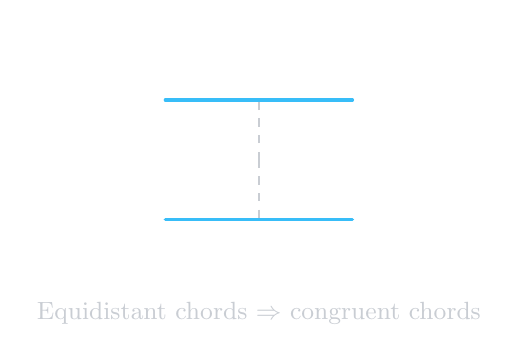
\begin{tikzpicture}[scale=0.95]
  \def\r{1.75}
  \coordinate (O) at (0,0);
  \coordinate (A1) at (-1.25,0.80);
  \coordinate (B1) at ( 1.25,0.80);
  \coordinate (A2) at (-1.25,-0.80);
  \coordinate (B2) at ( 1.25,-0.80);
  \coordinate (M1) at ($(A1)!0.5!(B1)$);
  \coordinate (M2) at ($(A2)!0.5!(B2)$);

  \draw[base] (O) circle (\r);
  \node[dot,label={[lab]below:$O$}] at (O) {};
  \draw[new] (A1)--(B1);
  \draw[new] (A2)--(B2);
  \draw[help] (O)--(M1);
  \draw[help] (O)--(M2);
  \node[labm] at (0,-2.05) {Equidistant chords $\Rightarrow$ congruent chords};
\end{tikzpicture}
\end{StepDiagram}
\[
\boxed{\text{(d) chords}}
\]
\end{QAPair}

% ============================================================
\begin{QAPair}{MCQ (viii)}
\textcolor{gold}{\bfseries Question:} Length of chord of a circle of radius $5$ cm is $8$ cm. The distance of chord from centre is:\\
(a) 3 cm \quad (b) 4 cm \quad (c) 5 cm \quad (d) 6 cm
\tcblower
\textcolor{green}{\bfseries Answer:}\par
\Step{1} Half-chord $=\dfrac{8}{2}=4$ cm.
\begin{StepDiagram}
\begin{tikzpicture}[scale=0.95]
  \def\r{1.75}
  \coordinate (O) at (0,0);
  \coordinate (A) at (-1.25,0.75);
  \coordinate (B) at ( 1.25,0.75);
  \coordinate (M) at ($(A)!0.5!(B)$);
  \draw[base] (O) circle (\r);
  \node[dot,label={[lab]below:$O$}] at (O) {};
  \draw[new] (A)--(B);
  \node[labfill] at ($(A)!0.5!(M)+(0,0.25)$) {$4$};
  \node[labfill] at ($(M)!0.5!(B)+(0,0.25)$) {$4$};
\end{tikzpicture}
\end{StepDiagram}

\Step{2} Use $d=\sqrt{r^2-\left(\frac{L}{2}\right)^2}$:
\[
d=\sqrt{5^2-4^2}=\sqrt{25-16}=3\text{ cm}.
\]
\EqDiagram{$d=\sqrt{25-16}=\sqrt{9}=3$}

\begin{StepDiagram}
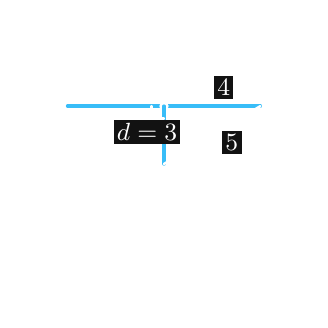
\begin{tikzpicture}[scale=0.98]
  \def\r{1.75}
  \coordinate (O) at (0,0);
  \coordinate (A) at (-1.25,0.75);
  \coordinate (B) at ( 1.25,0.75);
  \coordinate (M) at ($(A)!0.5!(B)$);
  \draw[base] (O) circle (\r);
  \node[dot,label={[lab]below:$O$}] at (O) {};
  \draw[new] (A)--(B);
  \node[dot] at (M) {};
  \draw[new] (O)--(M);
  \draw[base] (O)--(B);
  \draw[base] ($(M)+(-0.16,0)$) -- ($(M)+(-0.16,-0.16)$) -- ($(M)+(0,-0.16)$);
  \node[labfill] at ($(O)!0.55!(M)+(-0.22,0)$) {$d=3$};
  \node[labfill] at ($(M)!0.62!(B)+(0,0.24)$) {$4$};
  \node[labfill] at ($(O)!0.56!(B)+(0.18,-0.14)$) {$5$};
\end{tikzpicture}
\end{StepDiagram}

\[
\boxed{\text{(a) }3\text{ cm}}
\]
\end{QAPair}

% ============================================================
\begin{QAPair}{MCQ (ix)}
\textcolor{gold}{\bfseries Question:} What is the radius of circle in the figure? (Chord $=24$ cm, distance from centre $=5$ cm)\\
(a) 26 cm \quad (b) 10 cm \quad (c) 5 cm \quad (d) 13 cm
\tcblower
\textcolor{green}{\bfseries Answer:}\par
\Step{1} Half-chord $=12$ cm.
\begin{StepDiagram}
\begin{tikzpicture}[scale=0.92]
  \def\R{1.85}
  \coordinate (O) at (0,0);
  \coordinate (A) at (-1.35,0.85);
  \coordinate (B) at ( 1.35,0.85);
  \coordinate (M) at ($(A)!0.5!(B)$);
  \draw[base] (O) circle (\R);
  \node[dot,label={[lab]below:$O$}] at (O) {};
  \draw[new] (A)--(B);
  \node[labfill] at ($(A)!0.5!(M)+(0,0.25)$) {$12$};
  \node[labfill] at ($(M)!0.5!(B)+(0,0.25)$) {$12$};
\end{tikzpicture}
\end{StepDiagram}

\Step{2} In right triangle, $r^2=5^2+12^2=169 \Rightarrow r=13$ cm.
\EqDiagram{$r^2=25+144=169 \;\Rightarrow\; r=13$}

\begin{StepDiagram}
\begin{tikzpicture}[scale=0.95]
  \def\R{2.05}
  \coordinate (O) at (0,0);
  \coordinate (A) at (-1.55,0.95);
  \coordinate (B) at ( 1.55,0.95);
  \coordinate (M) at (0,0.95);

  \draw[base] (O) circle (\R);
  \node[dot,label={[lab]below:$O$}] at (O) {};
  \draw[new] (A)--(B);
  \node[dot,label={[lab]above:$M$}] at (M) {};
  \draw[new] (O)--(M);
  \draw[base] ($(M)+(-0.18,0)$) -- ($(M)+(-0.18,-0.18)$) -- ($(M)+(0,-0.18)$);
  \node[labfill] at ($(O)!0.5!(M)+(-0.35,0)$) {$5$};
  \node[labfill] at ($(M)!0.6!(B)+(0,0.25)$) {$12$};
\end{tikzpicture}
\end{StepDiagram}

\[
\boxed{\text{(d) }13\text{ cm}}
\]
\end{QAPair}

% ============================================================
\begin{QAPair}{MCQ (x)}
\textcolor{gold}{\bfseries Question:} In the figure, $AB=4$ cm, $OC=3$ cm. Chord $DE$ passes through midpoint of $OC$ and is parallel to $AB$. Find $DE$.\\
(a) 4.5 cm \quad (b) 5.6 cm \quad (c) 6.6 cm \quad (d) 3.3 cm
\tcblower
\textcolor{green}{\bfseries Answer:}\par

\Step{1} For chord $AB$, half-chord $=\dfrac{4}{2}=2$ cm. Hence radius:
\[
r^2=OC^2+2^2=3^2+2^2=13 \Rightarrow r=\sqrt{13}.
\]
\EqDiagram{$r=\sqrt{13}$}

\begin{StepDiagram}
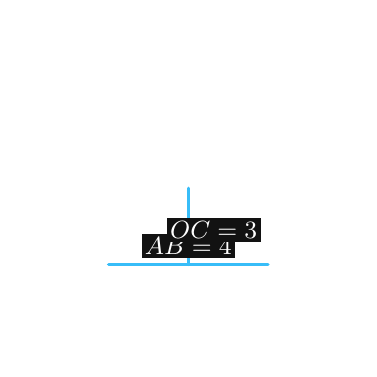
\begin{tikzpicture}[scale=0.92]
  \def\R{2.2}
  \coordinate (O) at (0,0);
  \coordinate (C) at (0,-1.05);
  \coordinate (A) at (-1.10,-1.05);
  \coordinate (B) at ( 1.10,-1.05);

  \draw[base] (O) circle (\R);
  \node[dot,label={[lab]above:$O$}] at (O) {};
  \node[dot,label={[lab]below:$C$}] at (C) {};
  \draw[new] (O)--(C);
  \draw[new] (A)--(B);
  \node[labfill] at ($(A)!0.5!(B)+(0,0.25)$) {$AB=4$};
  \node[labfill] at ($(O)!0.55!(C)+(0.35,0)$) {$OC=3$};
\end{tikzpicture}
\end{StepDiagram}

\Step{2} Midpoint of $OC$ is at distance $d=\dfrac{3}{2}=1.5$ cm from $O$.
\EqDiagram{$d=\dfrac{3}{2}=1.5$}

\begin{StepDiagram}
\begin{tikzpicture}[scale=0.92]
  \def\R{2.2}
  \coordinate (O) at (0,0);
  \coordinate (C) at (0,-1.05);
  \coordinate (M) at (0,-0.525);
  \draw[base] (O) circle (\R);
  \node[dot,label={[lab]above:$O$}] at (O) {};
  \node[dot,label={[lab]below:$C$}] at (C) {};
  \node[dot,label={[lab]right:$M$}] at (M) {};
  \draw[new] (O)--(C);
  \node[labfill] at ($(O)!0.55!(M)+(0.38,0)$) {$d=1.5$};
\end{tikzpicture}
\end{StepDiagram}

\Step{3} Chord length at distance $d$:
\[
DE=2\sqrt{r^2-d^2}=2\sqrt{13-1.5^2}
=2\sqrt{10.75}=\sqrt{43}\approx 6.56\text{ cm}.
\]
\EqDiagram{$DE=\sqrt{43}\approx 6.56\text{ cm} \Rightarrow \text{closest option }6.6\text{ cm}$}

\begin{StepDiagram}
\begin{tikzpicture}[scale=0.92]
  \def\R{2.2}
  \coordinate (O) at (0,0);
  \coordinate (C) at (0,-1.05);
  \coordinate (A) at (-1.10,-1.05);
  \coordinate (B) at ( 1.10,-1.05);
  \coordinate (M) at (0,-0.525);
  \coordinate (D) at (-1.55,-0.525);
  \coordinate (E) at ( 1.55,-0.525);

  \draw[base] (O) circle (\R);
  \node[dot,label={[lab]above:$O$}] at (O) {};
  \node[dot,label={[lab]below:$C$}] at (C) {};
  \node[dot,label={[lab]right:$M$}] at (M) {};

  \draw[new] (O)--(C);
  \draw[new] (A)--(B);
  \draw[new] (D)--(E);

  \node[labm] at (0,-2.55) {$DE$ is closer to $O$ than $AB$, so $DE>AB$};
\end{tikzpicture}
\end{StepDiagram}

\[
\boxed{\text{(c) }6.6\text{ cm}}
\]
\end{QAPair}

% ============================================================
\begin{QAPair}{MCQ (xi)}
\textcolor{gold}{\bfseries Question:} An angle whose vertex is centre of circle and whose arms pass through end points of an arc is known as \_\_\_\_\_ angle.\\
(a) inscribed \quad (b) central \quad (c) interior \quad (d) exterior
\tcblower
\textcolor{green}{\bfseries Answer:}\par
\Step{1} Vertex at the centre $\Rightarrow$ \textbf{central angle}.
\begin{StepDiagram}
\begin{tikzpicture}[scale=0.92]
  \def\R{1.65}
  \coordinate (O) at (0,0);
  \coordinate (A) at (\R,0);
  \coordinate (B) at ({\R*cos(55)},{\R*sin(55)});
  \draw[base] (O) circle (\R);
  \node[dot,label={[lab]below:$O$}] at (O) {};
  \draw[new] (O)--(A);
  \draw[new] (O)--(B);
  \pic[ang,"central",lab,angle radius=9mm,angle eccentricity=1.12] {angle=A--O--B};
\end{tikzpicture}
\end{StepDiagram}
\[
\boxed{\text{(b) central}}
\]
\end{QAPair}

% ============================================================
\begin{QAPair}{MCQ (xii)}
\textcolor{gold}{\bfseries Question:} Corresponding arcs of two congruent chords of a circle are \_\_\_\_\_.\\
(a) unequal \quad (b) major \quad (c) congruent \quad (d) minor
\tcblower
\textcolor{green}{\bfseries Answer:}\par
\Step{1} Equal chords subtend equal arcs $\Rightarrow$ arcs are \textbf{congruent}.
\begin{StepDiagram}
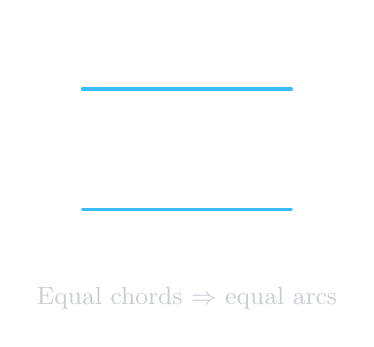
\begin{tikzpicture}[scale=0.90]
  \def\R{1.7}
  \coordinate (O) at (0,0);
  \coordinate (A) at ({\R*cos(30)},{\R*sin(30)});
  \coordinate (B) at ({\R*cos(150)},{\R*sin(150)});
  \coordinate (C) at ({\R*cos(210)},{\R*sin(210)});
  \coordinate (D) at ({\R*cos(330)},{\R*sin(330)});
  \draw[base] (O) circle (\R);
  \draw[new] (A)--(B);
  \draw[new] (C)--(D);
  \node[labm] at (0,-2.1) {Equal chords $\Rightarrow$ equal arcs};
\end{tikzpicture}
\end{StepDiagram}
\[
\boxed{\text{(c) congruent}}
\]
\end{QAPair}

% ============================================================
\begin{QAPair}{MCQ (xiii)}
\textcolor{gold}{\bfseries Question:} Length of two arcs (in the ratio $1:3$) and central angle of one arc is $60^\circ$, the second arc is \_\_\_\_\_.\\
(a) minor \quad (b) major \quad (c) semicircle \quad (d) circle
\tcblower
\textcolor{green}{\bfseries Answer:}\par
\Step{1} Arc length $\propto$ central angle, so angles are in ratio $1:3$.
\Step{2} Second central angle $=3\times 60^\circ=180^\circ$ $\Rightarrow$ a \textbf{semicircle}.
\begin{StepDiagram}
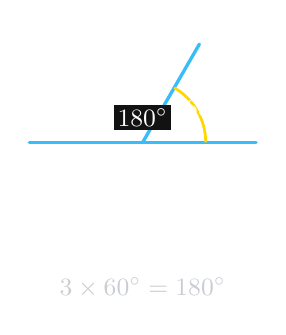
\begin{tikzpicture}[scale=0.90]
  \def\R{1.6}
  \coordinate (O) at (0,0);
  \coordinate (A) at (\R,0);
  \coordinate (B) at ({\R*cos(60)},{\R*sin(60)});
  \coordinate (C) at (-\R,0);

  \draw[base] (O) circle (\R);
  \node[dot,label={[lab]below:$O$}] at (O) {};

  \draw[new] (O)--(A);
  \draw[new] (O)--(B);
  \pic[ang,"$60^\circ$",lab,angle radius=8mm,angle eccentricity=1.12] {angle=A--O--B};

  \draw[new] (O)--(C);
  \node[labfill] at (0,0.35) {$180^\circ$};
  \node[labm] at (0,-2.05) {$3\times 60^\circ=180^\circ$};
\end{tikzpicture}
\end{StepDiagram}
\[
\boxed{\text{(c) semicircle}}
\]
\end{QAPair}

% ============================================================
\begin{QAPair}{MCQ (xiv)}
\textcolor{gold}{\bfseries Question:} The central angle of quadrant of a circle is \_\_\_\_\_.\\
(a) $30^\circ$ \quad (b) $45^\circ$ \quad (c) $60^\circ$ \quad (d) $90^\circ$
\tcblower
\textcolor{green}{\bfseries Answer:}\par
\Step{1} A quadrant is one-fourth of a circle: $\dfrac{360^\circ}{4}=90^\circ$.
\begin{StepDiagram}
\begin{tikzpicture}[scale=0.90]
  \def\R{2.1}
  \coordinate (O) at (0,0);
  \coordinate (A) at (\R,0);
  \coordinate (B) at (0,\R);
  \draw[base] (O) circle (\R);
  \draw[new] (O)--(A);
  \draw[new] (O)--(B);
  \node[dot,label={[lab]below:$O$}] at (O) {};
  \pic[ang,"$90^\circ$",lab,angle radius=10mm,angle eccentricity=1.12] {angle=A--O--B};
\end{tikzpicture}
\end{StepDiagram}
\[
\boxed{\text{(d) }90^\circ}
\]
\end{QAPair}

% ============================================================
\begin{QAPair}{MCQ (xv)}
\textcolor{gold}{\bfseries Question:} If a circle is divided into ten equal arcs, then central angle of each arc is \_\_\_\_\_.\\
(a) $10^\circ$ \quad (b) $36^\circ$ \quad (c) $60^\circ$ \quad (d) $90^\circ$
\tcblower
\textcolor{green}{\bfseries Answer:}\par
\Step{1} $\dfrac{360^\circ}{10}=36^\circ$.
\EqDiagram{$360^\circ \div 10 = 36^\circ$}
\begin{StepDiagram}
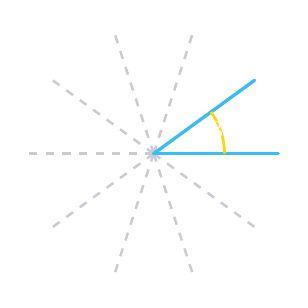
\begin{tikzpicture}[scale=0.88]
  \def\R{1.8}
  \coordinate (O) at (0,0);
  \draw[base] (O) circle (\R);
  \node[dot,label={[lab]below:$O$}] at (O) {};
  \foreach \k in {0,36,...,324}{
    \draw[help] (O)--({\R*cos(\k)},{\R*sin(\k)});
  }
  \coordinate (A) at (\R,0);
  \coordinate (B) at ({\R*cos(36)},{\R*sin(36)});
  \draw[new] (O)--(A);
  \draw[new] (O)--(B);
  \pic[ang,"$36^\circ$",lab,angle radius=9mm,angle eccentricity=1.12] {angle=A--O--B};
\end{tikzpicture}
\end{StepDiagram}
\[
\boxed{\text{(b) }36^\circ}
\]
\end{QAPair}

% ============================================================
\begin{QAPair}{MCQ (xvi)}
\textcolor{gold}{\bfseries Question:} How many central angles of an arc can be drawn?\\
(a) one \quad (b) two \quad (c) finite \quad (d) infinite
\tcblower
\textcolor{green}{\bfseries Answer:}\par
\Step{1} For a fixed arc (fixed endpoints), radii to endpoints form \textbf{one} central angle.
\begin{StepDiagram}
\begin{tikzpicture}[scale=0.92]
  \def\R{1.75}
  \coordinate (O) at (0,0);
  \coordinate (A) at ({\R*cos(20)},{\R*sin(20)});
  \coordinate (B) at ({\R*cos(120)},{\R*sin(120)});
  \draw[base] (O) circle (\R);
  \node[dot,label={[lab]below:$O$}] at (O) {};
  \node[dot,label={[lab]right:$A$}] at (A) {};
  \node[dot,label={[lab]left:$B$}] at (B) {};
  \draw[new] (O)--(A);
  \draw[new] (O)--(B);
  \pic[ang,"one",lab,angle radius=9mm,angle eccentricity=1.12] {angle=A--O--B};
\end{tikzpicture}
\end{StepDiagram}
\[
\boxed{\text{(a) one}}
\]
\end{QAPair}

% ============================================================
\begin{QAPair}{MCQ (xvii)}
\textcolor{gold}{\bfseries Question:} Two congruent chords of two congruent circles have \_\_\_\_\_ central angles.\\
(a) different \quad (b) same \quad (c) proportional \quad (d) acute
\tcblower
\textcolor{green}{\bfseries Answer:}\par
\Step{1} Congruent circles + congruent chords $\Rightarrow$ equal (same) central angles.
\begin{StepDiagram}
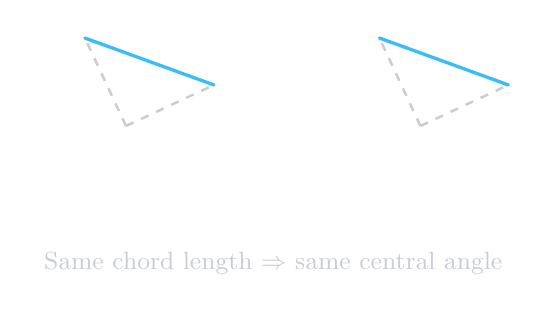
\begin{tikzpicture}[scale=0.85]
  \def\R{1.45}
  \coordinate (O1) at (-2.2,0);
  \coordinate (O2) at ( 2.2,0);
  \draw[base] (O1) circle (\R);
  \draw[base] (O2) circle (\R);
  \node[dot,label={[lab]below:$O_1$}] at (O1) {};
  \node[dot,label={[lab]below:$O_2$}] at (O2) {};

  \coordinate (A1) at ($(O1)+({\R*cos(25)},{\R*sin(25)})$);
  \coordinate (B1) at ($(O1)+({\R*cos(115)},{\R*sin(115)})$);
  \coordinate (A2) at ($(O2)+({\R*cos(25)},{\R*sin(25)})$);
  \coordinate (B2) at ($(O2)+({\R*cos(115)},{\R*sin(115)})$);

  \draw[new] (A1)--(B1);
  \draw[new] (A2)--(B2);

  \draw[help] (O1)--(A1);
  \draw[help] (O1)--(B1);
  \draw[help] (O2)--(A2);
  \draw[help] (O2)--(B2);

  \node[labm] at (0,-2.05) {Same chord length $\Rightarrow$ same central angle};
\end{tikzpicture}
\end{StepDiagram}
\[
\boxed{\text{(b) same}}
\]
\end{QAPair}

% ============================================================
\begin{QAPair}{MCQ (xviii)}
\textcolor{gold}{\bfseries Question:} Central angle of an arc which includes a semicircle in it is \_\_\_\_\_.\\
(a) $<90^\circ$ \quad (b) $>90^\circ$ \quad (c) $<180^\circ$ \quad (d) $>180^\circ$
\tcblower
\textcolor{green}{\bfseries Answer:}\par
\Step{1} If an arc includes a semicircle, it is a \textbf{major arc}, so its central angle is \textbf{more than $180^\circ$}.
\begin{StepDiagram}
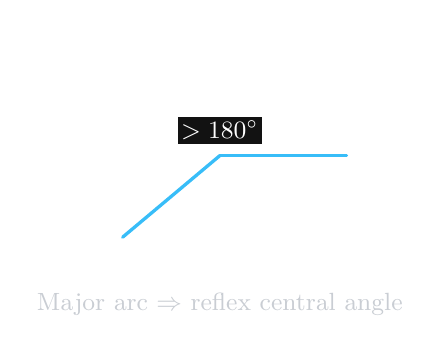
\begin{tikzpicture}[scale=0.92]
  \def\R{1.75}
  \coordinate (O) at (0,0);
  \coordinate (A) at (\R,0);
  \coordinate (B) at ({\R*cos(220)},{\R*sin(220)});
  \draw[base] (O) circle (\R);
  \node[dot,label={[lab]below:$O$}] at (O) {};
  \draw[new] (O)--(A);
  \draw[new] (O)--(B);
  \node[labfill] at (0,0.35) {$>180^\circ$};
  \node[labm] at (0,-2.05) {Major arc $\Rightarrow$ reflex central angle};
\end{tikzpicture}
\end{StepDiagram}
\[
\boxed{\text{(d) } >180^\circ}
\]
\end{QAPair}

\end{document}
